\chapter{Data Preparation}
generell diagramm with steps 

\begin{figure}[H]
	\centering
	\begin{tikzpicture}[node distance = 4cm, auto]
	% Place nodes
	\node [block] (matrix) {Create similarity matrix for glare effect};
	\node [block, right of=matrix, node distance=5cm] (mapping) {Mapping};
	\node [block, right of=mapping, node distance=5cm] (valid) {Valid logs collection};
	\node [block, below of=matrix] (quality) {quality plotting};
	\node [block, below of=mapping] (sorting) {Sorting of logs};
	\node [block, below of=valid] (simulate) {Simulation};
	\node [decision, below of=quality, node distance=4cm] (decide) {Are simulated logs realistic?};
	\node [block, below of=simulate] (change) {Change simulator};
	\node [block, below of=decide] (generate) {Generate features};
	\node [block, below of=change] (train) {Proceed with traning};
	
	% Draw edges
	\path [line] (matrix) -- (mapping);
	\path [line] (mapping) -- (valid);
	\path [line] (valid) -- (simulate);
	\path [line] (simulate) -- (sorting);
	\path [line] (quality) -- (decide);
	\path [line] (sorting) -- (quality);
	\path [line, pos=0.12] (decide) -- node {No}(change);
	\path [line] (change) -- (simulate);
	\path [line] (decide) -- node [midway] {Yes}(generate);
	\path [line] (generate) -- (train);
	
	\end{tikzpicture}
	\caption[Bild kurz]{hi}
\end{figure}

It would have been possible if the simualtions for glare effcet are fundamentally wrong to go back to the beginning and change the approch of creating the similarity matrix or find a new approch. However, the simualtinos of glare effect were very good, which can be seen in \todo{ref}, which is why the spproach was kept and not changed. Further training was not done with all iterations. Only with first and last one for comparison. 



\section{Similarity matrix creation}

%\section{Glare effect similarity matrix}
%\subsection{Matrix generation}
\subsection{Conceptualization}
The aim is to create a similarity matrix that descibes the differneces between colours under the influence of the simulated sun light. The difficulty hereby is that the intensity of the light is not spread evenly across the whole field. Instead, as it would be if a real sun would shine onto the display, a certain are has the highest intensity and the intensity is lower the further away from that area. Adittionally there are wide lines of higher intensity comming from the brightest area, that simulate sunbeams. This influence of the simulated sunlight can be seen in figute \ref{fig:glareEffect}. 

\begin{figure}[H]
	\centering
	
\includegraphics[width=15cm]{images/glareEffect.png}
	\caption[Bild kurz]{Screenshot of the game field with simulated sunlight. Sunbeams are especially visible on the right hand side. All cards are turned face up.}
	\label{fig:glareEffect}
\end{figure}

As a result simply extracting the rgb values for one pixel of each card in one game and calculating the differneces has two major problems: Firstly, the differences are highly influenced by the position of the specific cards. For instance might light green and yellow only be seperable for the human eyes if not direclty in the area of the brighhtest light. Secondly, extracting single pixels for each card in an image could lead to color values that do not represent the overall observed colour due to varying brightnesses on differnet points of a card. This behaviour is undesired, as the final similarity matrix is supposed to represent the differneces of the observed colours of the cards. \todo{vielleicht quelle suchen die sagt das menschen farbenm ion bereichen mitteln oder so} In order to solve these problems a more complex approach then simply extracting single pixels out of a game was needed. \\\\
The problem of the positional influence can be solved by using more than one game for corcaluating the color differences and taking the means differneces. \todo{besser beschrieben wie gesamtes idee, delta e color differnece} The idea is that by creating using so many games that all or most combinations of positions and colours are included and calculating the mean of all comparissons for , the result will not be influenced by the position of the cards. However, first needs to be determined which number of games satisfies this condition. Each game consists of 14 cards, with each two cards having the same colours. When determining the difference between two colours there are two differnet cases: 
\begin{itemize}
	\item 1. The colours are not the same: In each game there are exactly 4 combinations of positions for those two colours, because there are two cards for each colour (comparing for instance green1 and yellow1, green1 and yellow2, green2 and yellow1 and green2 and yellow2). 
	\item 2. The colours are the same: In each game there is only one combination of positions for those colours (comparing green1 and green2).  
\end{itemize}

\begin{figure}[H]
	\centering
	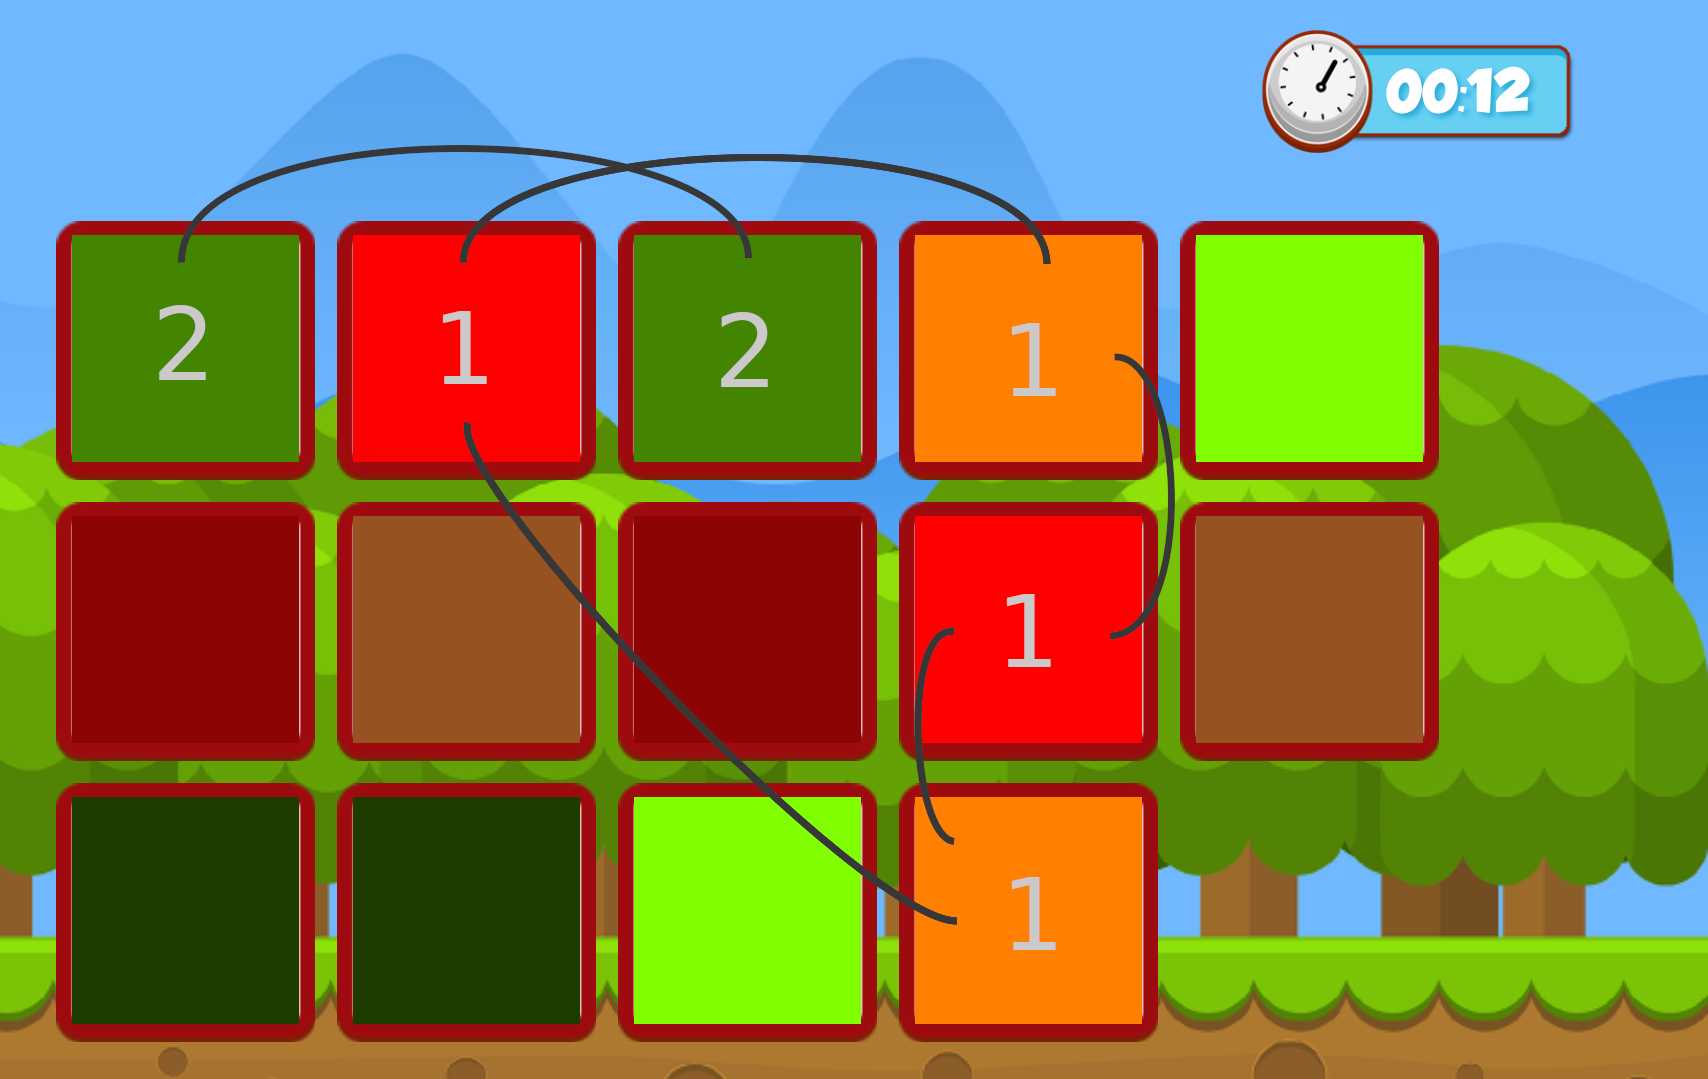
\includegraphics[width=15cm]{images/noObstTurnedNotes.png}
	\caption[Bild kurz]{Examplary showing the number of different comparissons for case 1 and 2. The numbers on the cards represent the case and the edges indicate unique comparissons. All cards are turned face up. A game without any obstacles is used only for the purpose of clarifying the differnet comparissons. All screenshots used for the actual calculation are taken from glare effect games.}
	\label{fig:noObstTurnedNotes}
\end{figure}

First it is calculated how many screenshots are necessary for the first case. For two different coloured arbitrary but fixed cards there can be 
\begin{equation*}
C\textsubscript{1} = 14 \cdot 13 = 182 
\end{equation*}
combinations of positions are possible. The reason that it is not not 14 $\cdot$ 14 is that 14 comparissons of cards with themself would be included. We formulate the condition that enough screenshots need to be taken so that a arbitrary but fixed combination of positions for two different colours is included with a probability of 95\%. 

\begin{center}
	As there are 4 such combinations of positions in each game the probanility P(A) to get a specific combination in a game is 
	\begin{equation*}
	P(A) = \frac{4}{182} % = 0.02198
	\end{equation*}
	The counter probability P($\lnot$A) is 
	\begin{equation*}
	P(\lnot A) = 1 - \frac{4}{182} = \frac{178}{182}%0.02198 = 0.97802
	\end{equation*}
	The number of necceary screenshots to include a specific combination with 95\% probaility is calculated by solving
	\begin{align*}
	1 - P(\lnot A)^n &\geq 0.95 \\
	1 - \left(\frac{178}{182}\right)^n &\geq 0.95 \\
	1 &\geq 0.95 + \left(\frac{178}{182}\right)^n\\
	\left(\frac{178}{182}\right)^n &\leq 0.05\\
	n &\geq log_{(\frac{178}{182})}(0.05) \\
	n &\geq 134.8024 %\llap{$\implies$\hspace{50pt}} at beginnging for implication arrow
	\end{align*}
\end{center}
This means that about 135 Screenshots of games are needed in the first case. Now we perform the same calculation for the second case where there is only one combination of positions for the colours. However, there are less combinations of positions that are relevant than in the first case. For example for two green cards at index 0 and 1 the 182 comparissons would include a comparison of the first green card and the second green card as well as a comparisson of the second green card and the first green card. This goes for every two cards with the same colour, meaning there are only half as many different comparissons in the second case than in the first case. As a result the number of possible combinations in the second case is
\begin{equation*}
C\textsubscript{2} = \frac{C\textsubscript{1}}{2} = \frac{14 \cdot 13}{2} = 91.
\end{equation*}
Now we calculate how many screenshots must be taken to include a specific combination of positions for two equal colours with a probability of 95\%. 
\begin{center}
	As there is one such combinations of positions in each game the probanility P(A) to get a specific combination in a game is 
	\begin{equation*}
	P(A) = \frac{1}{91} % = 0.02198
	\end{equation*}
	The counter probability P($\lnot$A) is 
	\begin{equation*}
	P(\lnot A) = 1 - \frac{1}{91} = \frac{90}{91}.%0.02198 = 0.97802
	\end{equation*}
	The number of necceary screenshots to include a specific combination with 95\% probaility is calculated by solving
	\begin{align*}
	1 - P(\lnot A)^n &\geq 0.95 \\
	1 - \left(\frac{90}{91}\right)^n &\geq 0.95 \\
	1 &\geq 0.95 + \left(\frac{90}{91}\right)^n\\
	\left(\frac{90}{91}\right)^n &\leq 0.05\\
	n &\geq log_{(\frac{90}{91})}(0.05) \\
	n &\geq 271.111 %\llap{$\implies$\hspace{50pt}} at beginnging for implication arrow
	\end{align*}
\end{center}
This means that about 272 screenshots of games are needed in the second case. As there are more screenshots needed for the second case, the first case is also included. This inclusion is caused by the fact that each screenshot includes comparissons for the  fist  as well as the second case. To have a buffer the decision was made to take screenshots of 300 games. In theory these screenshot include any arbitrary but fixed combinations of positions and colours with a probability of over 95\%.\\\\
To assure that these screenshots actually include most of the combinations and therefore eliminate the positional influence of cards, the coverage of combinations can be additionally calculated. Therefore the number of unique combinations included in the 300 screenshots must be divided by the overall number of possible combinations. The number of unique combinations can be counted during the process of creating the similarity matrix, but the number of possible combinations must seperatly determined. The similarity matrix for glare effect has 28 entries, from which 7 are comparissons between same and 21 between different colours. With \textit{C\textsubscript{1}} and \textit{C\textsubscript{2}}  being the possible combinations for two arbitrayry but fixed coloured cards in the two cases mentioned above, the number of overall possible combinations C is
\begin{align*}
C &= 21 \cdot C\textsubscript{1} + 7 \cdot C\textsubscript{2}\\
&= 21 \cdot 182 + 7 \cdot 91\\
&= 4459. 
\end{align*}
Furthermore is was verified that certain combinations are not included significantly more often than others and in that sense have stronger influence on the result. This was not the case ...\todo{code ergänzen und nachprüfen wie oft die combinationen vorkamen..histogramm?}. \\\\
Nonetheless, this does not solve the second problem of extracting single pixels that can potentially be directly in the area of a sunbeam. This can be fixed, by extracting all pixels in a certain are of the card and averaging their rgb values. %By averaging all colours in a certain area, the result will be more representitive of what the player actually sees \todo{Quelle finden wo sowas über visuellen kram gesagt wird}. 

\subsection{Screenshot extraction}
To play the memory game and take screenshots an emulator for the pixel 2 in android studio was used. In order to take the screenshots in the needed way and collect additionally necessary information some changes to the memory game were made. In the way the game is intended there are always only maximum two cards turned face up. However, for the screenshots all cards need to be turned around so that the colour differneces can be calculated. Therefore the memory game was adjusted so that all cards are turned face up once the player turns a card. Additionally it was changed so that cards stay face up once they get turned around for the first time. This makes it possible to take screenshots with the colours of all cards visible. Furthermore, for the creation of the similarity matrix it needs to be known what the original colours without the influnece of the simulated sun are. To collect the screenshots and the according colours of the cards in each game a semi-automatic approach was chosen. Once a game is started and a card is flipped, resulting in all cards being turned face up, the colours of all cards are saved in a list. Then a screenshot is manually taken and afterwards the game is exited to enter the main menu. From there on the process is repeated 300 times. As a result there are 300 hundred screenshots of games and a two dimensional list that includes the colours of the cards in the 300 games. The first dimension specifies the game and the second dimension the index of the card. The values of this list are stored in a text file before the game is completely closed. To assure that no mistakes were made when taking the screenshots, the number of collected screenshots is observed during the whole process and afterwards all screenshots are manually checked so that all cards are turned face up.

\subsection{Implementation}
This section will show and explain the implementation of the similarity matrix generation. Not every line of code will be included, but rather the most important parts. First of all the screenshots and the information about the original colours of the cards are loaded. Before the actual calculation of a similarity matrix for each image, the average rgb values of the cards on the field need to be determined. 
\begin{lstlisting}[language=python, caption=Add caption]
def determine_glare_rgb_values(image):
'''
Calculates the rgb average rbg values for each card in an image.
:param image: The screenshot of the memory game with all cards 
turned face up.
:return: The average rbg values in the specified 150 x 150 pixel 
areas for each card. 
'''
glare_rgb_values = []
for corner in card_corners:
x_border = corner[0] + 150
y_border = corner[1] + 150
card_values = []
for x in range(corner[0], x_border, 1):
for y in range(corner[1], y_border, 1):
coordinates = x, y
pixel_values = image.getpixel(coordinates)
card_values.append(pixel_values[:-1])
card_r = int(round(np.mean([color[0] for color in card_values])))
card_g = int(round(np.mean([color[1] for color in card_values])))
card_b = int(round(np.mean([color[2] for color in card_values])))
glare_rgb_values.append((card_r, card_g, card_b))
return glare_rgb_values 
\end{lstlisting}
The cards are each 250 $\cdot$ 250 pixels big and the rgb values are extracted from squared 150 $\cdot$ 150 pixel areas. The coordinates the pixels are extracted from are manually selected in gimp. As a result the areas are only correct for the used resolution of 1080p. Once the mean rgb values in those areas are calculated the similarity matrix can be created. Each of the 28 cells in the similarity matrix falls into one of the two cases explained in \todo{ref}, meaning there are either 4 or only 1 unique combination for the calculation of each cell value. For every combination the lab colour distance is determined and the values for each cell are averaged. This completes the steps for a single image, resulting in a similarity matrix with unscaled values. 
%\begin{lstlisting}[language=python, caption=Add caption]
%def determine_distance(color_1_rgb, color_2_rgb):
%	'''
%	Determines dinstance between colors with delta e formula. 
%	:param color_1_rgb: The first color.
%	:param color_2_rgb: The second color.
%	:return: The delta_e distance between the two colours. 
%	'''
%	lab_1 = convert_color(color_1_rgb, LabColor)
%	lab_2 = convert_color(color_2_rgb, LabColor)
%	
%	if cie_1976:
%		detlta_e = delta_e_cie1976(lab_1, lab_2)
%	else:
%		detlta_e = delta_e_cie2000(lab_1, lab_2, Kl=1, Kc=1, Kh=1)
%	return detlta_e
%\end{lstlisting}
Once a similarity matrix for every image is created, the average of all matrices is calculated. During the whole calculation of the single matrices it is being kept track of the highest occurring colour differnece. The last step neccessary to complete the final similarity matrix is to use the highest colour differnce to scale all values down to be between 0 and 1. 

Through the original colours loaded in the beginning, the coverage of combinations in the 300 games can be calculated. 
\begin{lstlisting}[language=python, caption=Add caption]
def determine_coverage(original_colors):
'''
For calculating how many of the combinations are includes 
in the calcuation. 
The calculations are based on having 14 cards on the field.
:param original_colors: A list containing tuples with the card name, 
the mappimg number for the card, and the index for each card on the 
screenshot for all screenshots.
:return: The coverage of combinations of positions 
for all colour combinations. 
'''|\Suppressnumber|

[...]|\Reactivatenumber{18}|

combinations = []
for colors in original_colors:
for i in range(len(colors)):
original_color_1 = colors[i]
for l in range(len(colors)):
original_color_2 = colors[l]
if original_color_1[2] != original_color_2[2] and (original_color_2, original_color_1) not in combinations and (original_color_1, original_color_2) not in combinations:
combinations.append((original_color_1, original_color_2))    
return len(combinations) / number_of_total_combinations
\end{lstlisting}

\subsection{Manual testing}
To verify the correcteness of the color extraction and the calculation of the similarity matrix, the main funtionalities are manually tested. The colour extraction was tested by extracting colours of a screenshot with the skript and compoaring the rgb values to the actual values in the images using gimp. Furthermore the calculation of the delta e score was tested, by comaring results of the script with those of an online calculator.  

\subsection{Final Matrix}
In figure \ref{fig:simMatrix} the final similarity matrix can be seen, dsiplaying how colour differneces are observed under the influence of the simulated sunlight, averaged over 300 games. As mentioned before, the lower the delta e score the more similar the cards appear to the human eye. 
\begin{figure}[H]
	\centering
	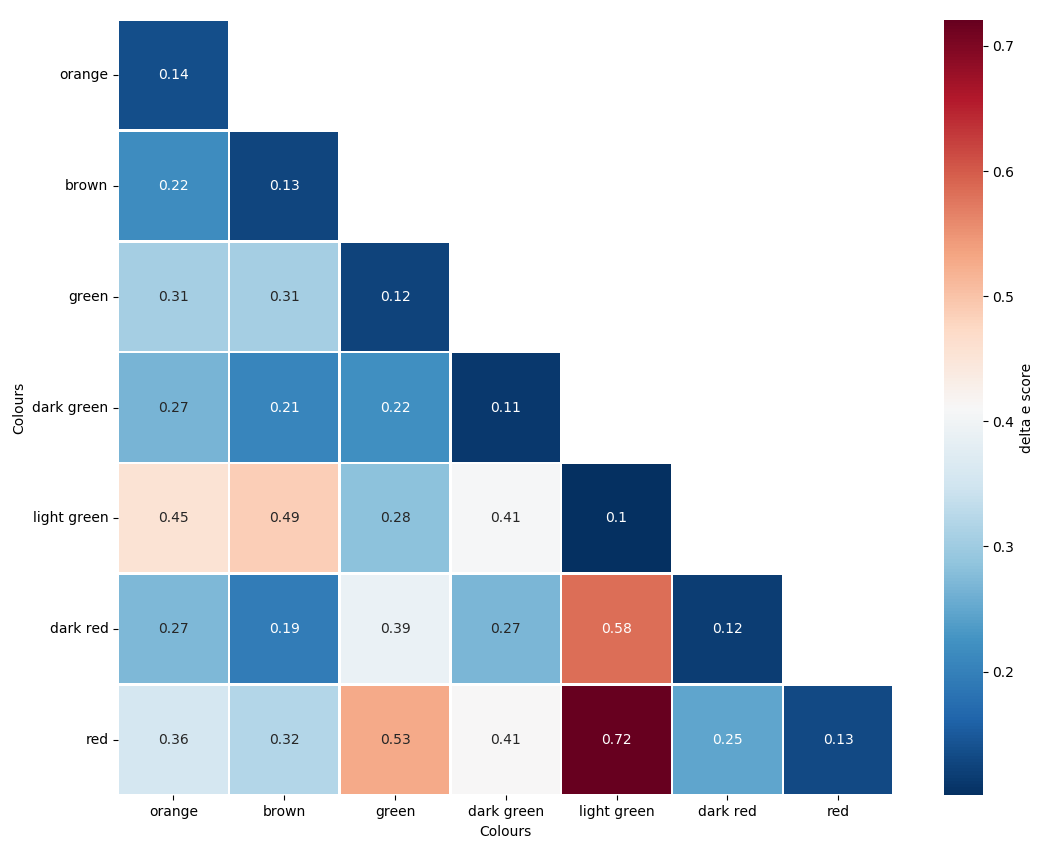
\includegraphics[width=15cm]{images/simMatrix.png}
	\caption[Bild kurz]{Add caption}
	\label{fig:simMatrix}
\end{figure}
The 300 games used for creating this matrix include 99.57\% of all possible combinations. Before actually using the constructed simialry matrix in the simulator it is unknown if the chosen approach results in high quality simulations. If this is not the case it is possible to change the concept or try other approches. 

\section{Adaptation and correction of logs}
- structure of logs and mapper that maps logs and replaces old matrix with new one\\
- methode für mapping bereits vorhanden, aber es mussten einige anpassungen gemacht werden und ergänzungen: neue matrix einfügen statt der alten, bentzte funktionen wurden nicht mehr unterstützt und mussten geändert werden, methode wurde in ein neues skript eingebaut welches das mapping für alle logs macht und das ergebnis in einer neuen datei speichert.\\
- was ich gemacht habe um zu überprüfen ob mapping nocfh korrekt ist: vergleichen von altem und neuen mapping 

\section{Removal of invalid logs}
For the simualation to work, the game log that is used for the simulation must have had all cards turned around at least once. Initially, this was not the case. Therefore a script was written that collects all no obstacle and all glare effect logs, validates them and saves only the valid ones in new files. It need to be noted, that if at least one the two logs from a participant is invalid, both logs are removed. Otherwise the training data could include no obstacle games but no glare effcect logs from a participant and vise versa, which should be avoided \todo{mehr erklären wieso das nicht gut ist und vielleicht quelle finden}. A log is invalid if not all cards were turned at least once. 
\begin{lstlisting}[language=python, caption=Add caption]
def validate_log(log):
'''
Validates logs.
:param log: The log to validate. 
:return: If the log is valid.
'''
needed_entries = ['1.1,', '2.1,', '3.1,', '4.1,', '5.1,', '6.1,', '7.1,', '1.2,', '2.2,', '3.2,', '4.2,', '5.2,', '6.2,', '7.2,']
for needed_entry in needed_entries:
if needed_entry not in log:
return False
return True
\end{lstlisting}

\section{Simulation of user behaviour}
Multiple additions were made to the simulator. In total four classes were added. Two are for generating configuration files for the simulation of game with and without the glare effect obstacle (NoObst\_ConfigGenerator\_dataCollection2020.java and GlareEffect\_ConfigGenerator\_dataCollection2020.java) and the other two for using those files to simulate new games based on the user behaviour in the original games (NoObstWinStrategyTrainingDataGenerator\_dataCollection2020.java and GlareEffectWinStrategyTrainingDataGenerator\_dataCollection2020.java). These classes utilize the functionalities already implemented in the simulator. \todo{Code grob für jeweils eine zeigen}



\section{Sorting logs by quality}
- wichtigh um beim training immer nur die besten n zu nehmen

\section{Evaluation of simulation}
- intial results\\
- problems\\
- chnages\\
- final results \\
- im realfall benutzen wir nicht alle simulationen sondern nur die besten. die werden vorher nach güte sortiert und dann nur die besten 1-10 und 20 genommen. Bilder zeigen wie es da aussieht bei finalem. \\
- resulkts show that the similarity matrix used creates very good simulations of glare effect games. \\
- t-stochastic test kram (siehe mazens nachricht)

\section{Feature generation}
- directory preperatrion\\
- feature creation\\
